\documentclass[a4paper, titlepage, 12pt]{article}
\usepackage[left=3cm, right=3cm, top=4cm, bottom=4cm]{geometry}
\usepackage[utf8]{inputenc}
\usepackage{color}
\usepackage{caption}
\usepackage{subcaption}
\usepackage{array}
\usepackage[hidelinks]{hyperref}
\usepackage{graphicx}
\usepackage[square,sort,comma,numbers]{natbib}
\usepackage{amsfonts}
\usepackage{bbm}
\usepackage{booktabs}
\usepackage{multirow}
\usepackage{amsmath}


% SET YOUR DATA HERE
% This is a preliminary title for your thesis.
\newcommand{\thesisTitle}{LDPC encoding hardware architectures for on-board processing datachains}

% Your full name.
\newcommand{\name}{Dimitrios Theodoropoulos ($\Delta 695$)}

% The time frame in which you want to write the thesis.
\newcommand{\timeFrame}{April 2016 - September 2021}

% The primary supervisor. You probably do not need to change this.
\newcommand{\supervisor}{Prof. Antonios Paschalis}

% The name(s) of your advisor(s). This is probably the PhD student or PostDoc that you are working with.
\newcommand{\advisor}{Prof. Dimitris Gizopoulos \\ Prof. Nektarios Kranitis}

% Select if this is a Bachelor or Master Thesis.
\newcommand{\thesisType}{PhD}


\newcommand\todo[1]{\colorbox{yellow}{#1}}
\setlength{\bibsep}{0.0pt}

\begin{document}

\begin{titlepage}
\begin{center}
\LARGE{\textbf{National and Kapodistrian University of Athens}}\\
\normalsize{Department of Informatics and Telecommunications}\\[0.3cm]

\begin{figure}[h!]
    \centering
    
\includegraphics[width=0.7\linewidth]{logo_el.png}
\end{figure}
\vspace{1cm}

\LARGE{{\thesisType} PhD Thesis}\\[0.7cm]
\Huge{\textbf{\thesisTitle}}

\vspace{1cm} 

\Large{\textbf{\name}} \\[3pt]  
\vspace{0.5cm}
\large{Time frame: \timeFrame} \\ 

\vspace{1cm}

\large{\textbf{Supervisor}}\\
\supervisor\\
\vspace{0.5cm}
\textbf{Advisor}\\
\advisor\\
\end{center}
\end{titlepage}
\tableofcontents
\clearpage
\section{Introduction}
\label{sec:intro}
\subsection{Forward Error Correction schemes}
Forward Error Correction (FEC) coding schemes are used extensively in almost every communication and data processing system, in order to increase the reliability of transmission and storage of data. This is especially important in space communications scenarios, due to the extremely stringent SNR requirements of deep-space links, or conversely, the high data rates and low latency necessary in near-earth satellite communication scenarios. At the same time, an efficient FEC scheme implementation in a realistic scenario has to balance contradicting requirements and offer a variety of trade-offs in terms of error correcting efficiency, encoding/decoding complexity, throughput, hardware resources utilization and power consumption.\par
The traditional approach which has been widely adopted since the dawn of digital communications implements countermeasures against errors caused by noise, distortion and interference,  at the symbol level. We refer to this component of the communication system as channel coding \cite{Ryan2009}. Almost every modern communication standard and system includes a channel coding scheme, at least as an option. Well known schemes in this area include Reed-Solomon (RS) \cite{Reed1960} and Turbo \cite{Berrou1993} codes. Another highly advantageous class of channel codes are the Low-Density Parity-Check (LDPC) codes, which are linear block codes, characterized by large block lengths and sparse parity-check matrices. Introduced by R.G. Gallager in 1960 \cite{Gallager1962}, LDPC codes had in following years generally succumbed to oblivion, due to the current era’s technology limitations, which could not allow their implementation at a reasonable cost. However, advances in VLSI technology, together with the application of efficient code design techniques have annihilated those barriers. Among the entire range of modern error correcting codes (ECC), they are currently the most promising approach towards the capacity limit described by Shannon \cite{Shannon}. This has established them as the optimal choice for FEC in modern applications.\par

The initial Gallager codes were random and although they exhibited excellent error-correcting capabilities, hardware implementation was challenging. In order to reduce implementation complexity and encoding/decoding speed, additional structure has been designed into the parity check matrices of all practical LDPC codes in modern applications, so that they consist of an array of juxtaposed cyclic sub matrices, named the circulants, which can be efficiently implemented. These structured codes are collectively referred to as Quasi-Cyclic (QC) LDPC codes. QC-LDPC codes have been adopted by many modern communication standards, such as IEEE 802.11, 802.16 and DVB-S2. A special class of structured LDPC codes, the protograph-based QC codes have recently received considerable research interest in many modern standards. QC LDPC codes have also been adopted by the Consultative Committee for Space Data Systems (CCSDS) as recommended standard for on-board channel coding in Near-Earth and Deep-Space communications \cite{CCSDS131.0}.\par
A multitude of encoder architectures for QC-LDPC codes has been proposed in the literature, while several products are available in the market. Most of the proposed architectures though are optimized for the specific codes adopted by corresponding standards, leveraging the specific properties if the particular code structure. Especially those demonstrating practical throughput in the range of multiple Gbps, they are either entirely not applicable or are not expected to scale with CCSDS codes, the parity-check matrix of which do not exhibit the required structure.\par

The error correcting capability of bit-level channel coding however is limited in high speed and deep fading scenarios, such as those encountered in modern earth-to-satellite and satellite-to-satellite laser links. Moreover, these environments are characterized by high latency and traditional automatic repeat request (ARQ) schemes are not applicable or practical, or the fading effect of the communication channel is so deep that bit-level channel codes cannot provide the required reliability, since even a single scintillation effect can span multiple entire transmitted codewords. In these cases, the erroneously received or completely missed codewords can be considered as erased symbols and the most suitable model for the communication channel is the block erasure channel. Error correction in this case takes place at a higher level of the communications protocol stack than bit-level channel coding (which is typically a function of the data link layer in OSI protocol stack). Erased symbols are entire packets of the underlying protocol.\par

A common approach for coding over block erasure channels is the combination of RS codes with interleaving. RS codes are maximum distance separable (MDS) codes: if $(n,k)$ are the dimensions of a code, it can recover from the erasure of any $n-k$ or fewer symbols. Consequently, they can provide optimal error recovery capability. An interleaver is typically connected to the output of the RS encoder in order to protect against deep fading. Such coding schemes have been proposed in \cite{CCSDS141} and \cite{CCSDS142} for optical space communications. The limitation of RS codes, however, is high encoding complexity, which imposes the use of short block lengths. The polynomial arithmetic operations involved in encoding and decoding operations result in non-linear encoding/decoding complexity, even in the base case proposed in \cite{Tang2020}. The use of RaptorQ codes has alternatively been proposed in \cite{Adhikary2020}.\par
Another promising approach is the use of packet-level LDPC erasure codes, according to which encoded symbols are entire blocks of information bits. Although these codes are not MDS, capacity approaching ensembles can perform very close to the Singleton bound \cite{GuilleniFabregas2006} and encoder and decoder complexity can scale linearly with block length. Packet-level LDPC erasure coding has also been proposed in \cite{CCSDS131.5} for near-earth and deep space communications.\par




\subsection{On-board data processing}\label{subsec:Onboard}
The stringent requirements of aerospace applications in terms of reliability and power call for a different approach, when considering on-board data processing equipment. Commercial devices, targeting hugely larger market shares and lower time to market,  cannot obviously meet these requirements. Processors in space are required to withstand harsh environmental conditions, mainly due to radiation effects. In addition, the risk margin of the disruption of the mission needs to be significantly lower. To meet these ends, the space industry has established the notion of Technology Readiness Level, and the relevant guidelines for ECSS are provided in \cite{ECSS-E-HB-11A}.\par
The degradation of the reliability of electronic systems manifests itself in two forms of errors in their operation. The most severe form refers to hard errors. These can happen as a consequence of the gradual or sudden degradation of the system caused by the accumulation or a surge of total ionizing dose (TID) or atomic displacement (Total Non Ionizing Dose-TNID or Displacement Damage-DD) \cite{Ecoffet2013}. Another kind of effects are transient phenomena which lead to so-called "soft errors" in the component's operation. When the error in the system is caused by the passage of a single particle, the event can be categorised as Single Event Effect (SEE). SEEs can lead to soft errors, for example Single Event Upsets \cite{George2019}, or hard, as is the case with Single Event Upsets (SEU) or Burnouts (SEB).\par
Depending on the type of the effect, various mitigation techniques are applied at various levels: from the physical layer, which refers to the semiconductor fabrication process up to the system level design. Devices employing these techniques are referred to as radiation tolerant, or radiation hardened devices. Radiation hardening aims to minimise the probability of radiation effect's occurrence in the first place, mostly by measures on the physical layer and their cost of radiation hardened can be significantly higher than that of their commercial counterparts. Radiation tolerance, on the other hand, assumes that radiation effects are bound to occur and aims at reducing the impact of radiation effects on the system's operation. ECC in the memories and buses is the fundamental radiation tolerance technique. A summary of mitigation techniques at various levels of design can be found in \cite{HUANG2019105} and the references therein.\par
The topic of mitigation techniques is widely covered in the literature. Consequently, we limit our brief description to the following techniques, which are more relevant to this work: Triple Modular Redundancy (TMR) and memory scrubbing. In a basic TMR sheme, three redundant circuits perform the same task on the same data. A majority vote process at the system's output can mask a failure in one of the circuits. Obviously, the cost of this approach is that it requires triple resources. Memory scrubbing, as the name implies, is a method to increase the integrity of data stored in a memory system. It requires that a method of ECC has been applied to the data written in the memory. Its contents are periodically retrieved, any errors are detected and corrected with the ECC and the result is written back to the memory. The frequency of the memory scans needs to be balanced, so that single errors are not accumulated and the ECC fails.\par
Typical on-board data handling systems are built around a central processor (OBC-On Board Data Computer), which is mostly responsible for telecommand functions and the coordination of the rest of the platform subsystems: telecommunication, telemetry, mass memory subsystems, sensors, instruments,  and payload processors. All these subsystems communicate through highly reliable communication links, typically MIL-STD-1553, or spacewire and spacefibre, which are described separately in Section \ref{subsubsec:spfi}. The Space Avionics Open Interface Architecture (SAVOIR) initiative is a move towards the standardization of space avionics and, among other products, it proposes a reference functional architecture reference model.\par
In the near future space computing technology is expected to converge more rapidly with terrestrial practices \cite{Furano2018}, so that, depending on the mission goals, the required balance between performance, resiliency and cost is met: as smaller payloads with a limited lifespan are becoming more popular, the requirements for space-qualified parts can be relaxed. The most extreme example of this scenario is the case with cubesats and nanosattelites in the "new space" emerging trend \cite{newspace}, the lifespan of which can be as small as a few days \cite{Oltrogge}. In this aspect, for non-mission critical functions and time-specific payloads, even the use of COTS equipment can be acceptable.\par


\subsection{Space communication channels, systems \& protocols}
near-earth and deep space channel modelling. Then about erasure channel 
Fundamentals: Capacity, FEC basics, channel models


\clearpage
\section{Background}
\label{sec:background}
\subsection{FPGAs in space}\label{subsubsec:fpga}
Initially, FPGAs implemented only auxiliary tasks and glue logic in a spacecraft system. The basic telemetry and flight control tasks are handled by specialized CPUs, which is the topic of subsection of \ref{subsubsec:cpu}. However, FPGAs have recently gained increased popularity for aerospace applications, due to the increased processing power and size, weight, power, and cost (SWAP-C), when compared to CPUs and GPUs \cite{Lentaris2018}. In addition,  While continuing to support these functions, FPGAs are widely used for embedded computing in Space. For example, in \cite{Tsigkanos2020}, a Hyperspectral Image Compression implementation for CCSDS 123.0-B1 recommended standard is introduced, which is built on a COTS SoC. FPGAs are the de-facto solution for demanding processing acceleration applications, like deep-learning algorithms in neural networs.\cite{Vidmar2021}.\par
There only a limited number of Radiation Hardened By Design (RHBD) FPGAs in the market. The most important device families are manufactured by Microsemi and Xilinx \cite{leon21}. A common feature of these families is that the configuration memory is SRAM, instead of flash, since the latter technology is susceptible to radiation effects \cite{Marinella21}, with an obvious impact on the cost. The products of both vendors share a rich mission heritage, an extensive overview of which is also provided in \cite{leon21}.\par
In addition to the standard hardening techniques, Microsemi PolarFire radiation tolerant FPGAs chips use Silicon-Oxide-Nitride-Silicon (SONOS) Non-Volatile (NV) technology \cite{sonos}, which provides immunity against SEU effects, in addition to low power. The physical layer manufacturing details of the SONOS technology, as well as its rad-hard attrbutes are widely covered in \cite{sonos}. TMR in the user logic, when required, is assured through suitable provisions from the bundled software (Libero sinplify).\par
On the other hand, the Xilinx SRAM radiation hardened FPGA range includes the legacy Virtex-4QV FPGA (90nm) device family, the Virtex-5QV FPGA (65nm) XQR5VFX130 device and the RT Kintex UltraScale (20 nm) XQRKU060 device, which is currently the state-of-the-art in terms of performance.\par
In both cases which offers a wide selection of RHBD FPGAs, which have a long heritage in space missions. With their vendors being based in the USA, however, all these products are subject to USA export controls, which adds insecurity to the European missions' planning. Recently, the NanoXplore family of RHBD devices has been introduced as a European solution, although it has not yet presence in space.\par
Interestingly, an emerging trend for extending the application area of commercial Xilinx ZynQ and ZynQ Ultrascale+ SoCs into aerospace applications has risen recently. A number of research activities has been focusing on the study of the susceptibility of the ZynQ-7000 series SoCs. The SEU behaviour of the ZynQ-7020 SoC's integrated ARM Processing System is the subject of the work in \cite{Hiemstra2015}. In \cite{Tambara15}, the authors present their results on heavy proton SEU testing of the same device, while \cite{Bezerra17} evaluates the SEE behaviour of the NINANO board used in EYE-SAT nanosatellite. The work in \cite{Vlagkoulis21} is the most complete analysis of the SEE behaviour of ZynQ-7000 series programmable logic and configuration memory under heavy ion irradiation. One of its major contributions is that it provides the tools for the design of efficient mitigation techniques, including effective ECC and configuration memory scrubbing. At the same time, a multitude of research activities incorporate these SoCs for aerospace applications. In \cite{Tsigkanos2020}, for example, we have introduced a high performance parallel implementation of an accelerator for the CCSDS 123.0-B-1 hyperspectral compression algorithm. This work leverages the resources of both the processing system and the programmable logic to deliver state-of-the-art throughput performance. The authors in \cite{Sabogal19} propose a hybrid convolutional neural network accelerator for semantic segmentation of image, which is widely used in space applications. Their work is evaluated on Xilinx ZynQ and ZynQ Ultrascale+ MPSoCs, while performing error injection and radiation-beam testing, in order to characterise the response of the proposed architectural framework in the presence of radiation phenomena. In all these cases, mostly soft techniques are used as mitigation measures. TMR effectiveness under heavy ion radiation is evaluated in \cite{Sanchez19} for a ZynQ 7000 SoC supporting a  CCSDS 121.090-B-2 compression IP core, demonstrating a 40\% increased Mean Time To Failure (MTTF). A rather complete study of the effectiveness of soft methods is presented in \cite{Kibar19}. The key takeaway is that for non mission critical systems, soft SEE mitigation techniques can provide the resilience required for space applications.\par
In DSCAL, the following boards are available and used in the scope of the current thesis:
\begin{itemize}
    \item The KCU105 evaluation board, built around the Kintex UltraScale XCKU040 device, which is the commercial equivalent of the radiation tolerant Kintex Ultrascale XQRKU060. Regarding the rest of the board's equipment, of notable interest are the two SFP+ cages, which were used for spacefibre integration and the 2 GB of DDR4 RAM memory.
    \item The ZC706 board, featuring a Zynq-7000 XC7Z045 SoC at speed grade 2, with two ARM Cortex-A9 MPCore hard processors. One SFP+ cage is also included. The board also includes 1 GB of DDR3 RAM connected to the processing system (PS) build around the two ARM processors (component memory), as well as 1 GB of DDR3 RAM for the programmable logic (SODIMM memory). Access to the two memories is independent (both memories can be accessed at the same time).
    \item The Zedboard, with the Zynq-7000 SoC XC7Z020. The board has no SFP+ connections, but it includes 512MB DDR3 memory connected to the processing system. Access to the memory space from the programmable logic can be provided from the ZynQ's PS AXI3 high performance (HP) ports, as detailed in Section 
\end{itemize}

\subsection{Space-grade CPUs}\label{subsubsec:cpu}
Similarly to what is described in Section \ref{subsubsec:fpga}, the requirements of CPUs are radically different between terrestrial and aerospace applications. Commercial CPUs, target hugely larger market shares, can meet lower time to market requirements and include advanced features and vastly higher performance. Not being able to withstand the harsh environmental conditions typically met in spaceflight, however, they fail to meet the reliability requirements of space missions. Space-qualified CPUs have therefore been developed to mitigate these issues. These CPUs are based on commercial Instruction Set Architectures (ISAs), so the cost of the ecosystem around them is reduced. The ecosystems includes hardware design processes and tools, as well as software tools for applications development. Historically, MIL-STD-1750 architecture \cite{MIL-STD-1750} dominated space missions, due to its already widespread adoption by military airborne computers. Quickly, however, following the evolution of commercial architectures, the market was dominated by SPARC and PowerPC. A pictorial overview of the historical evolution of space CPUs is provided in Fig.\ref{fig:CPU-Archs}. 
	\begin{figure}
		\centering
		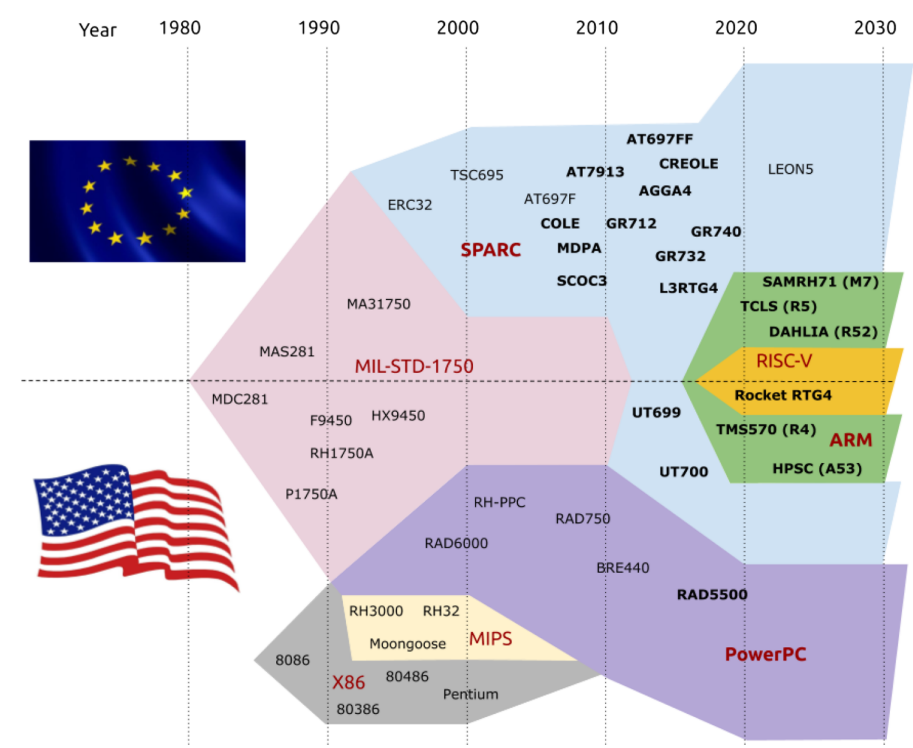
\includegraphics[width=0.6\linewidth]{Figures/CPUsHistory.png}
		\caption{History of CPU architectures used in space missions. Source: \cite{DiMascio2020}}
		\label{fig:CPU-Archs}
	\end{figure}
The European Space Agency (ESA) opted for the SPARC architecture, mainly because of the widespread availability of software and its open architecture, which allowed the Agency's independence from specific vendors. To this aim, ESA funded the development of the LEON processor in late 1997. One of the principal objectives of the project was the integration of fault tolerant-by-design techniques. The processor should be able to detect and tolerate one error in any register without software intervention, and to suppress effects from  Single Event Transient (SET) errors in combinational logic \cite{Anrersson2010}. LEON evolved in the following years and currently, LEON3 \cite{leon3} is the most widely adopted platform for ESA missions. LEON3 is distributed as synthesizable VHDL model of a 32-bit processor compliant with the IEEE-1754 (SPARC V8) architecture by Aeroflex Gaisler. The distribution is under the GNU GPL license allowing use for any purpose without licensing fee. The most significant upgrades over the previous LEON2 is the support of Symmetric Multi Processing (SMP) and pipelined operation at 5 stages. In space missions, a fault-tolerant version of the processor (LEON3FT) is the one that is widely used. Fault tolerance is assured by the implementation of ECC coding of all on-hip RAM blocks, which is able to detect and correct up to four errors per 32-bit RAM words or per cache memory tag, and all these without performance impact (completely transparent to user applications). The main means for achieving fault-tolerance is by using ECC coding of all on-chip RAM blocks. A famous LEON3-based SoC is the GR712RC from Aeroflex Gaisler.\par 
LEON5 is the latest version of  the LEON processor family\cite{leon5} and it primarily targets high-end FPGA's. Although it has not yet been implemented in space missions, it provides backward compatibility for most of the software implementations that have targeted LEON3 and LEON4 processors, claiming up to 85\% higher performance. Nevertheless, the Reduced Instruction Set Computer version V (RISC-V) Instruction Set Architecture (ISA) is expected to dominate upcoming on-board processing applications \cite{DiMascio2020}. In European missions for example, the De-RISC project \cite{derisc2020} has recently shown the first milestones for a multi-core RISC-V processor for aerospace designs. The project is based on the NOEL-V 64-bit RISC-V processor core \cite{noelv} from Aeroflex Gaisler and state-of-the-art hypervisor technology to accomplish high performance workloads, on a complete processing platform for space. The three processor models (LEON3/5, NOEL-V) are distributed as parts of the open-source GRLIB IP library, which is an integrated set of reusable IP cores, designed for system-on-chip (SoC) development and they are available also in fault-tolerant versions for FPGA and ASIC implementations. Typically, they are interconnected through Advanced Microcontroller Bus Architecture (AMBA) Advanced High-performance Bus (AHB) and Advanced Peripheral Bus (APB) interfaces. A typical SoC built around a single LEON/NOEL processor core with the peripherals included in the distribution is depicted in Fig. \ref{fig:LEONSoC}\par
	\begin{figure}
		\centering
		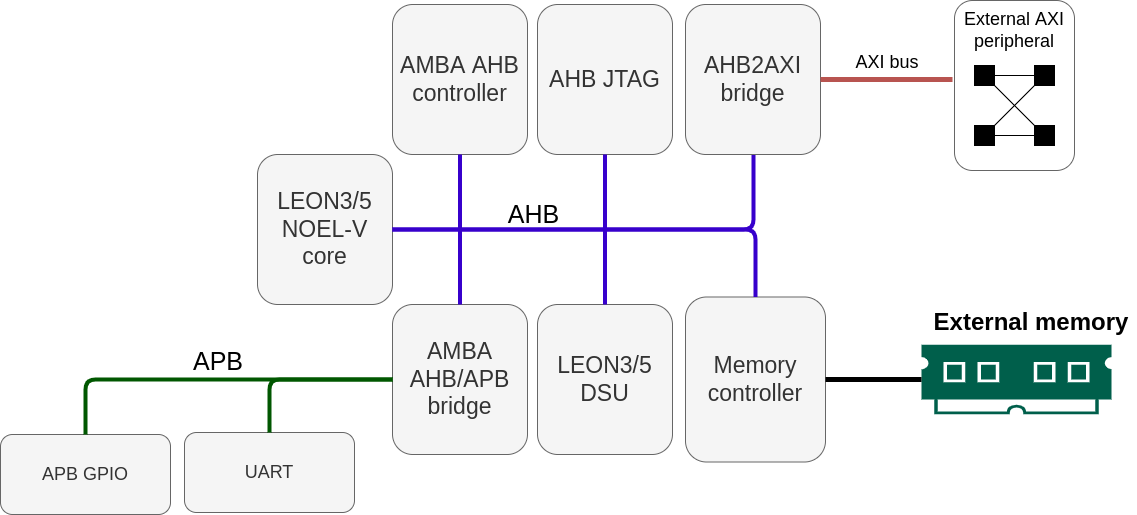
\includegraphics[width=0.8\linewidth]{Figures/LEONSoC.png}
		\caption{A typical LEON/NOEL SoC design}
		\label{fig:LEONSoC}
	\end{figure}
As its name implies, the AHB JTAG component shown in the image provides a JTAG debug link to the SoC, allowing among other things the uploading and debugging of user software to the processor's memory, through the GRMON software tool, which is part of the processor's software ecosystem. Other useful software tools included in the ecosystem are the cross-compiler for the CPU architecture and a simulator (TSIM). The debugging capabilities are completed with the Debug Support Unit (DSU) depicted in the image. This module communicates with the CPU through a dedicated debug interface (in addition to AHB) and has complete control over its pipeline, its registers and the contents of the instruction trace buffer. The processor can be set into debug mode by the DSU, which halts the pipeline. As part of the current work, the LEON/NOEL ecosystem has been set up on the KCU105 and Zedboard development board, to allow for interaction with custom FPGA peripherals, as well as for software comparison\par


\subsection{Spacewire and spacefibre}\label{subsubsec:spfi}
On-board processing systems examples are instruments, mass-memory, processors, and downlink telemetry. The interconnection of this systems is a challenging task:fault-tolerance, error recovery capabilities, low power, simplicity, performance and architectural flexibility place stringent requirements on the design of an on-board network. The interconnections of the equipment in such a network is feasible only with serial links. \cite{Athavale2005}.\par
Initially, space agencies and manufacturers followed their proprietary approaches to address this issue. The diversity of communication links that arose resulted in high cost, limited development and test time and interoperability issues. In 1992, the demand for interconnection of distributed signal-processing systems led ESA to assign the development of a new standard to the University of Dundee \cite{Parkes2012}. This process resulted in the first version of ECSS-E-ST-50-12C (SpaceWire) standard \cite{spwire}.
The standard defined a high speed data-handling on-board network and technology. It provides bidirectional, full-duplex data-links at speeds of 2 Mbit/s to 200 Mbit/s, which connect together SpaceWire enabled equipment. Data-handling networks can be built to suit particular applications using point-to-point data-links and routing switches.\par
	\begin{figure}
		\centering
		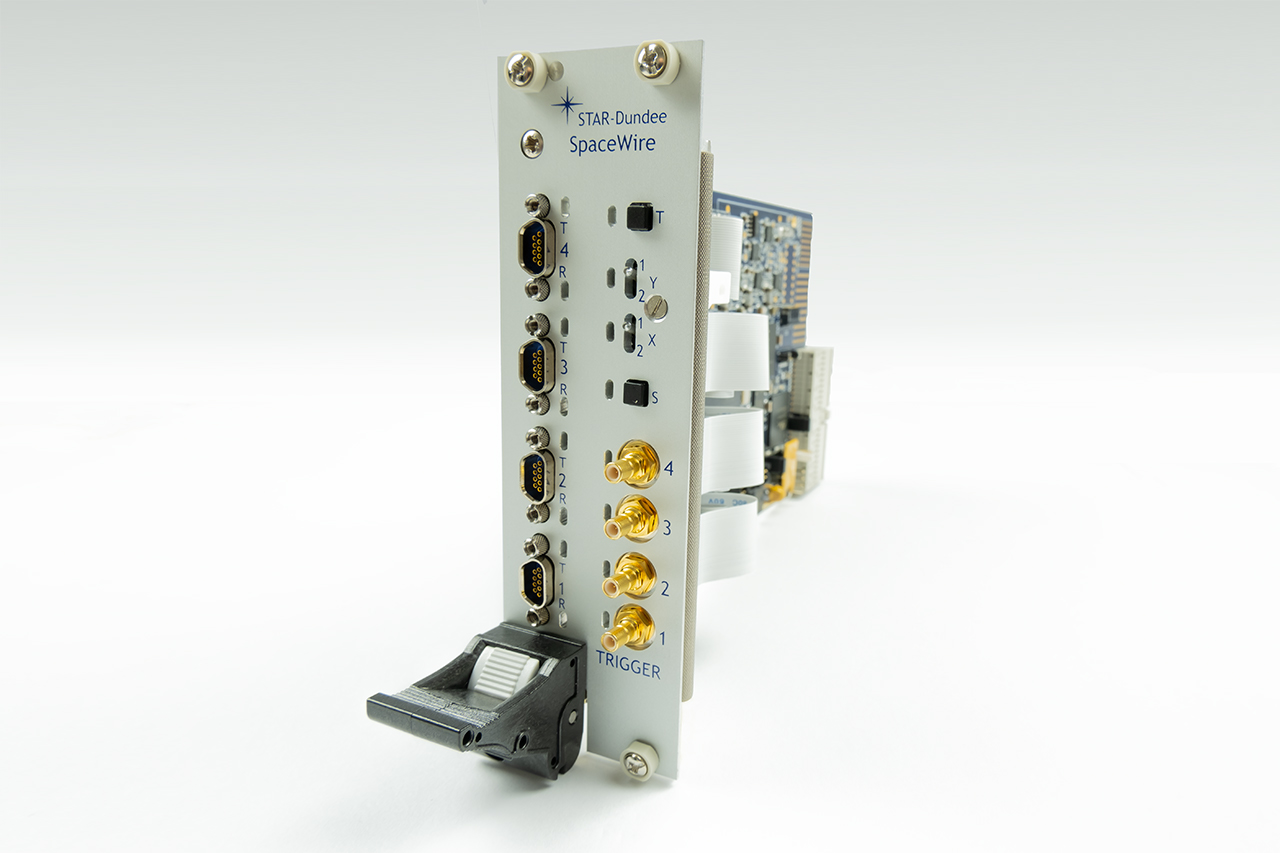
\includegraphics[width=0.5\linewidth]{Figures/pxi_interface_8hp_front.jpg}
		\caption{SpaceWire PXI Mk2 card from STAR-Dundee. (source: https://www.star-dundee.com/products/spacewire-pxi-mk2/)}
		\label{fig:A}
	\end{figure}
The next generation of SpaceWire is the SpaceFibre technology, standardised as ECSS-E-ST-50-11C \cite{spfibre}. Except for higher data rates (6,25 Gbps signalling rated), SpaceFibre comes with other significant enhancements:
\begin{itemize}
    \item Fibre-optic cabling, with electrical support for backwards compatibility with SpaceWire.
    \item Multi-laning, which can combine the throughput of multiple physical links (lanes) to support well over 20 Gbit/s.
    \item Advanced Quality of Service (QoS) mechanisms, like prioritization of Virtual Channels, bandwidth reservation and support of deterministic delivery constraints.
\end{itemize}
DSCAL is a partner of the Hi-SIDE project (https://www.hi-side.space/) consortium and as such, it has been granted a access to SpaceFibre test equipment, featuring a STAR-Ultra PCIe interface and link analyzer card (https://www.star-dundee.com/products/star-ultra-pcie), along with the necessary software tools (GUI and API for the development of custom applications and performance measurements). An accompanying encrypted IP core netlist, adds transparency in the communication of the software channel interface on the host PC's application with the logic implemented on an FPGA. The core exposes up to 7 AXI4-Stream 128-bit interfaces to the user logic and a RMAP port for configuration and control.\par
The provided equipment can provide two 4-lane SpaceFibre links to a suitable corresponding interface of up to 20 Gbit/s per link, depending on the number of SFP interfaces of the available FPGA platforms. The maximum data rate can be achieved when all four 6,25 Gbit/s lanes are used. Because of the 8b/10b encoding on the SpaceFibre link, only 80\% of the lane bandwidth is available to the user logic. Of the equipment available at DSCAL, only the Zynq UltraScale+ MPSoC ZCU102 development board with 4 SFP+ connector cases can support the maximum data rate of 20 Gbit/s. The ZCU105 card, however, which has been extensively used in this work can only provide up to 10 Gbit/s of user bandwidth.\par
	\begin{figure}
		\centering
		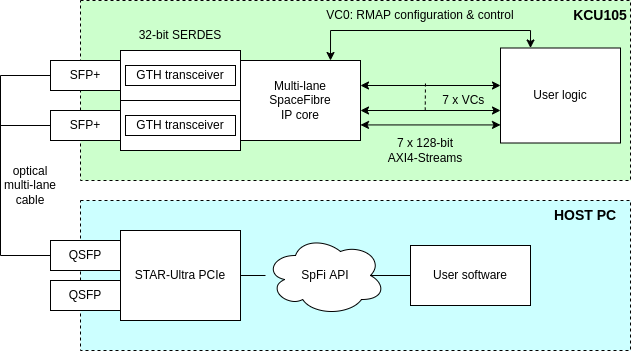
\includegraphics[width=0.6\linewidth]{Figures/SpFibre.png}
		\caption{Block diagram of the SpaceFibre equipment and environment}
		\label{fig:equipment}
	\end{figure}
As part of the Hi-Side project's deliverables, a sample design for the KCU105 had been provided to DSCAL. The reference design included a basic demo for a loopback test through the card's FMC connectors, without connectivity to the host PC. The reference design had to be modified, so that SERDES is mapped to the transceivers allocated to the SFP+ connectors of the board. The transceivers needed also to be parametrized and a suitable clock source to be configured on the board and connected to the transceivers' CPLLs. This process was different for the equipment used in DSCAL: the KCU105 and ZCU102 boards use GTH transceivers, while ZC706 uses GTX transceivers. Figure \ref{fig:equipment} is a block diagram of the resulting environment used for testing. The design depicted refers to the configuration used on the KCU105 board, but except for the number of lanes and type of transceivers, it is the same for all the other boards.\par
	\begin{figure}
		\centering
		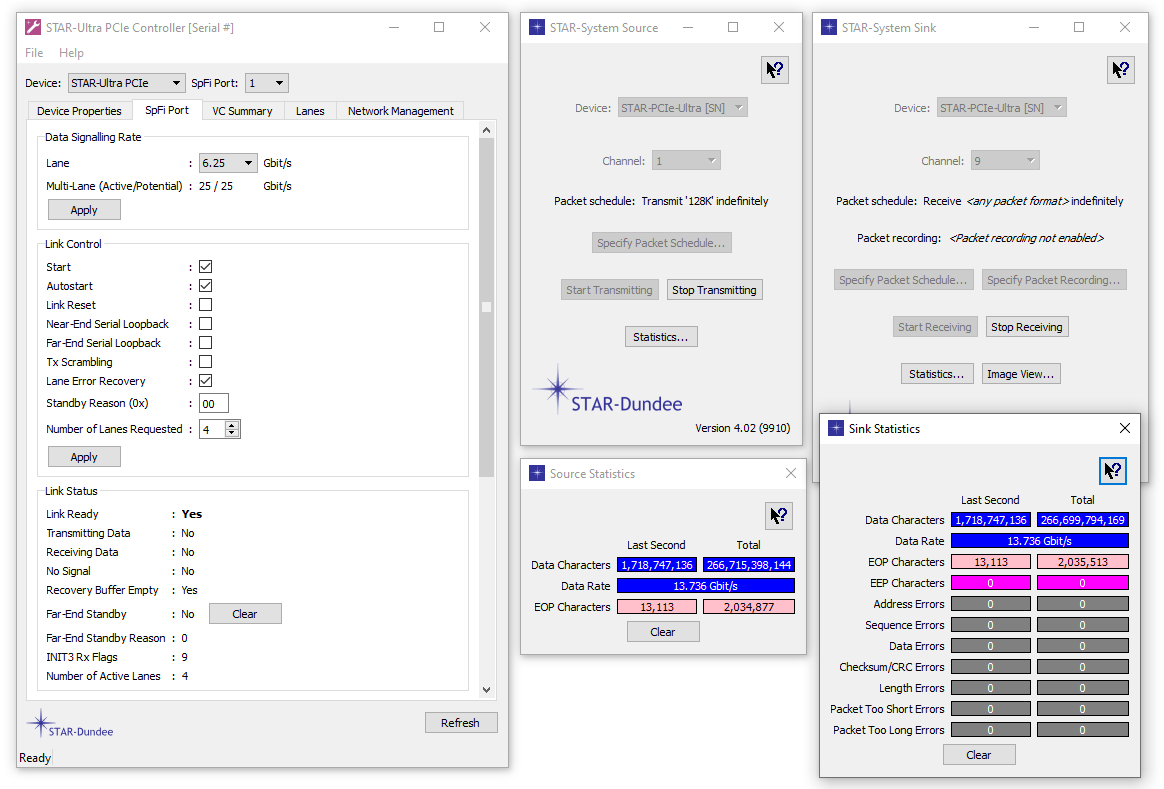
\includegraphics[width=0.6\linewidth]{Figures/star-ultra_pcie_tx_and_rx.png}
		\caption{GUI applications examples}
		\label{fig:gui}
	\end{figure}
On the PC side, the STAR-System software provided as part of the Hi-SIDE equipment provides the drivers of the SpaceFibre STAR-Ultra PCIe board, as well as the software tools for transmitting and receiving packets to and from the SpaceFibre IP code. The software bundle provides two options: a set of GUI applications and a complete API for the development of custom software tools. In both cases, statistics and performance data can be derived. Figure \ref{fig:gui} gives an example of the GUI applications. In order to streamline the automatic execution of scripts including SpaceFibre transactions, the following custom applications were developed, based on the STAR-System API:
\begin{itemize}
    \item rmapRead $<address>$: reads a 4-byte register at a user-specified address.
    \item rmapWrite $<address> <value>$: writes a 32-bit value at a register at a user-specified address.
    \item sendFile -c $<channel> -i <file>$: sends a binary file to the specified channel of the master stream interface of the core.
    \item sendFile -c $<channel> -i <file>$: receives data from the specified channel until an End Of Packet (EOP) character is sent and writes the stream into a file.
\end{itemize}

\subsection{Bit-level channel coding}
partial recofiguration on xupv5
testing with matlab model
\subsection{Magnetic recording media coding}
\subsection{Packet-level coding}
Do not forget to add the memory subsystem we created for LEON on ZynQ system (access to DDR memory through

\clearpage
\section{Review of the state-of-the-art}
\label{sec:related-work}
\subsection{QC LDPC bit-level codes}
In general, LDPC encoding refers to the process of calculating the mapping $s \rightarrow c$ of a k-bit binary vector $s\in\{\mathbb{F}_2\}^k$ to the proper element $c$ of the k-dimensional subspace $V\subset\{\mathbb{F}_2\}^n$, according to the code definition, which is defined by the parity-check matrix $H$ of the code, so that the parity-check equation $ cH^{T}=0 $ is satisfied.\par
The encoding methods for LDPC codes can be classified into the following categories:\par
\textbf{\textit{Direct method}}\par
The direct method involves the application of Gaussian elimination to calculate the generator matrix $G$ from the null space of the parity-check matrix $H$ of the code, that is to solve the equation $GH^{T}=0 $. This process takes place offline and depending on the encoder's implementation details, the generator matrix data or structure is stored into the encoder. A codeword $c$ can thus be calculated from the input information block $s$ through the vector-matrix multiplication $c=sG$.\par
In order to facilite encoder design, for all the practical LDPC codes used in modern communications systems, the generator matrix can be calculated in systematic form. For a $(n,k)$ linear block code in this case $G=\begin{bmatrix}I_{k} & W_{n-k}\end{bmatrix} $, where $I_{k}$ is the $k\times k$ identity matrix and for QC codes, $W_{n-k}$ is an array of dense cyclic sub-matrices, with the structure of (\ref{eq:Wstructure}). The resulting codeword $c$ is consequently $c=\begin{bmatrix}s & p\end{bmatrix}$, where $p$ is the vector of the $n-k$ parity bits. In this case, the encoders implementing this method need only to store the $r \times c \times m$ bits of the first rows (or columns) of these circulants. However, despite the fact that the initial parity-check matrix $H$ is sparse, the resulting $W_{n,k}$ matrix and consequently its constituent circulants are dense matrices. In \cite{Mahdi2014}, \cite{Wang2008} and \cite{Lee2004} compression methods are proposed, which reduce the memory requirements to store the circulants of the parity-check matrix $H$ in the encoder. These methods however are not applicable to dense matrices, nor are the corresponding architectures which handle the sparse matrix operations involved in the calculations.\par  
\begin{equation}
    W_{n-k}=
    \begin{bmatrix}
        W_{1,1} & \dots  & W_{1,c} \\
        \vdots  & \ddots & \vdots \\
        W_{r,1} & \dots  & W_{r,c}
    \end{bmatrix}
    \label{eq:Wstructure}                   
\end{equation}
Encoders proposed in \cite{Theodoropoulos2016},\cite{ZhaohuiWangXinHaoChangxingLin2018},\cite{Miles2006},\cite{ZongwangLi2006},\cite{Andrews2005},\cite{Yasotharan2009},\cite{Yen2012}  are based on the direct encoding method. My preliminary  work in \cite{Theodoropoulos2016} has introduced an efficient architecture for the parallel execution of the vector-matrix multiplication involved in the direct encoding method, by leveraging the inherent parallelism of the generator matrix of CCSDS codes, achieving.\par
Although the work in \cite{ZhaohuiWangXinHaoChangxingLin2018} focuses in CCSDS codes, the proposed architecture handles encoding inefficiently, requiring large XOR operations over a significant number of bits ($k/2$ or 2048 in the provided example) and at the same time register resources are wasted. Algorithmically, the approach is also equivalent to \cite{Yasotharan2009} and the parallel SRAA of \cite{ZongwangLi2006}. The required logic resources for hardware implementation are inevitably a large portion of a Virtex7-xc7vx485t FPGA.\par
In \cite{Miles2006}, the problematic dimension of the C2 code at the boundaries of the 511-bit circulants when processing a stream of input data is handled by packing input bits present on the 16-bit input bus into groups of 21-bits and unpacking them subsequently to groups of 7 bits for the AND-XOR operations. The difference however between the size of the input bus (16 bits) and the degree of parallelism in the AND-XOR process (MAC module), leads to suboptimal use of the resources of the MAC module, which remains idle for a number of cycles, when input has starved. Moreover, additional computation cycles are wasted by the 18 trailing zeros which are prepended to the information block, according to C2 code description, which are processed by the MAC module in this particular approach. Our architectures handle these problems in a more efficient way, as described in a subsequent section.\par
The authors in \cite{ZongwangLi2006} propose various types of encoding circuits, based on shift registers, which achieve encoding complexity linearly proportional to the number of parity bits of the code ($n-k $ according to the notation in this work), or the $n$ total bits of the code in the case of the parallel approach. The SRAA serial encoding scheme described is practically the naive approach provided in the CCSDS standard \cite{CCSDS131.0}, based on a shift register for the circulants and a register for the calculation of parity bits. The calculated complexity does not include the memory and the necessary circuitry for the loading of the generators $g_{i,j}$ of the circulants to the SRAA shift registers, which incur significant resources cost in practical implementations, as it will be shown in a subsequent section. According to the parallel SRAA approach, which achieves encoding in $cb$ cycles (following the writers' notation), all $k$ input bits participate in the calculation of each parity bit in one clock cycle. This architecture could not be implemented with reasonable resources in practical encoders for codes with block lengths in the range of several thousands of bits and should be considered only as a theoretical approach for academic research purposes only. Even in this case however, the AND-XOR binary calculations on a large number of bits would necessitate large combinatorial paths and would severely jeopardize throughput performance. The two-stage encoding scheme described is practically the \textit{H2-inverse} method described later in the current Section.\par
The work in \cite{Andrews2005} proposes an architecture based on Linear Feedback Shift Registers (LFSRs). The input information bits are multiplied with the first rows of the circulants $W_{i,j}$ and instead of rotating the circulant registers, the rotation concerns the output register, which contains the parity bits at the end of the encoding process.\par
The approach described in \cite{Yasotharan2009} is algorithmically equivalent to the parallel SRAA approach of \cite{ZongwangLi2006}, without taking advantage of the QC structure of the targeted codes (IEEE 802.16e). Its performance however is also dominated by the large XOR binary operation involved. In addition, the memory requirements for the storage of the generator matrix, totalling $(n-k)k$ bits, pose considerable constrains to the associated hardware. Finally, \cite{Yen2012} is another adoption of the SRAA architecture of \cite{ZongwangLi2006} employing the direct method, optimized for sparse circulants.\par

\textbf{\textit{R-U method}}\par
This method is based on the fact that the codeword can be calculated directly from the H matrix by solving the system of equations defined by the parity-check equation $Hc^{T}=0$. The Richardson-Urbanke (R-U) method \cite{Richardson2001} solves this equation with complexity almost linear to the block length, provided that the parity-check matrix of the corresponding QC-LDPC code has approximate upper-triangular structure, or it can be  transformed to such form, which is depicted in Fig.\ref{fig:RUmatrix}. For a systematic code with a $H$ matrix of size $(n-k)\times k$, the calculated codeword has the form $c=\begin{bmatrix}s & p_{1} & p_{2} \end{bmatrix}$, where $s$ is the input vector and $p_{1}$, $p_{2}$ are parity bits vectors of length $g$ and $m-g$ respectively and and the parity bits are calculated according to (\ref{eq:RUphi}), (\ref{eq:RU1}), (\ref{eq:RU2}).\par
\begin{figure}
    \centering                            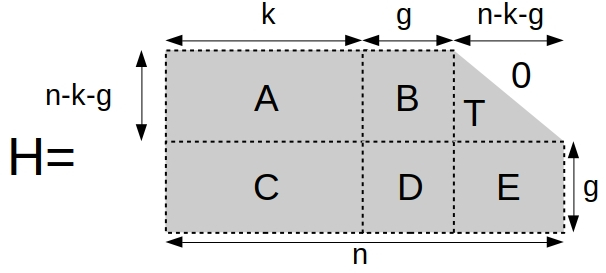
\includegraphics[width=0.4\linewidth]{Figures/RUmatrix.jpg}
    \caption{Structure or H matrix for the R-U method}
    \label{fig:RUmatrix}
\end{figure}
\begin{equation}
    \varphi=ET^{-1}B+D
    \label{eq:RUphi}
    \end{equation}
\begin{equation}
    p_1^{T}=\varphi^{-1}(ET^{-1}A+C)s^{T}
    \label{eq:RU1}
    \end{equation}
\begin{equation}
    p_{2}^{T}=T^{-1}(As^{T}+Bp_1^{T})
    \label{eq:RU2}
\end{equation}

The above equations involve many sparse matrices, but only a single dense, namely $\varphi^{-1}$. Sparse matrix operations can be implemented by simplified hardware and the determinant factor affecting the performance of the encoder becomes the $g \times g$ dense matrix $\varphi^{-1}$. The parity-check matrix of many widely adopted LDPC codes has been specifically designed so that the parameter $g$ is small, or in the case of DVB-S2 is zero and the matrix $\varphi^{-1}$ has a special strucutre which results in efficient hardware implementation. For example, the $\varphi$ matrix of the LDPC codes adopted for IEEE 802.11ac/n, 802.16e and many other applications is the $g \times g$ identity matrix.\par
For many other codes, transformation into approximate lower triangular form, without affecting the QC structure of the matrix is not straightforward. For example, in the case of the CCSDS codes defined in \cite{CCSDS131.0}, this can be achieved by shifting the last 4 circulants ($4m$ bits) by 8 columns ($8m$ bits) to the left. Since the last $4m$ bits of the code are punctured, this permutation does not affect the encoder's output. Fig.\ref{fig:RUH} displays the $H$ matrix before and after the transformation for rate $1/2$ AR4JA code with $k=1024$. The parameter $g$ is therefore $4m$ and $\varphi^{-1}$ is a $4m \times 4m$ dense QC matrix of $m \times m$ circulants.             
Architectures proposed in \cite{Lee2004}, \cite{Tzimpragos2013}, \cite{HaoZhong2005}, \cite{Yu2014}, \cite{Wang2017}, \cite{HaibinZhang2008} are examples of application of the R-U method.\par
          The work in \cite{Lee2004} does not target QC codes, nor can it efficiently handle large dense $\varphi$ matrices. The parameter $g$ is 2 in the provided implementation examples and the resulting encoders occupy a large amount of the resources of Xilinx XC2V4000-6 FPGA, including a number of Block RAMS. The encoder architecture in \cite{Tzimpragos2013} targets IEEE 802.11n codes where $\varphi$ matrix is the identity matrix, but is not applicable to CCSDS codes. Targeting Wimax LDPC codes, \cite{Wang2017} also assumes that $\varphi$ is the identity matrix. In \cite{HaoZhong2005} the authors propose a code construction method, together with encoder-decoder architectures. The proposed encoder implements the R-U method, but the code construction aims at minimizing the parameter $g$. The dense matrix multiplication (\ref{eq:RU1}) involving $\varphi$ in their case is executed on all elements of $\varphi^{-1}$ in parallel, which obviously does not scale efficiently for large $g$. The method proposed in \cite{HaibinZhang2008} and \cite{Yu2014} employs SRAA modules introduced in \cite{ZongwangLi2006} for the dense matrix operations of the RU algorithm. The scalability issues concerning the adoption of SRAA architectures for the direct encoding method, also petrain to the R-U method for CCSDS codes, because of the size of parameter $g$.\par
          %             Fig \ref{fig:phiInv} gives an example for the matrix of the same code. \par 
                \begin{figure}
                \centering
                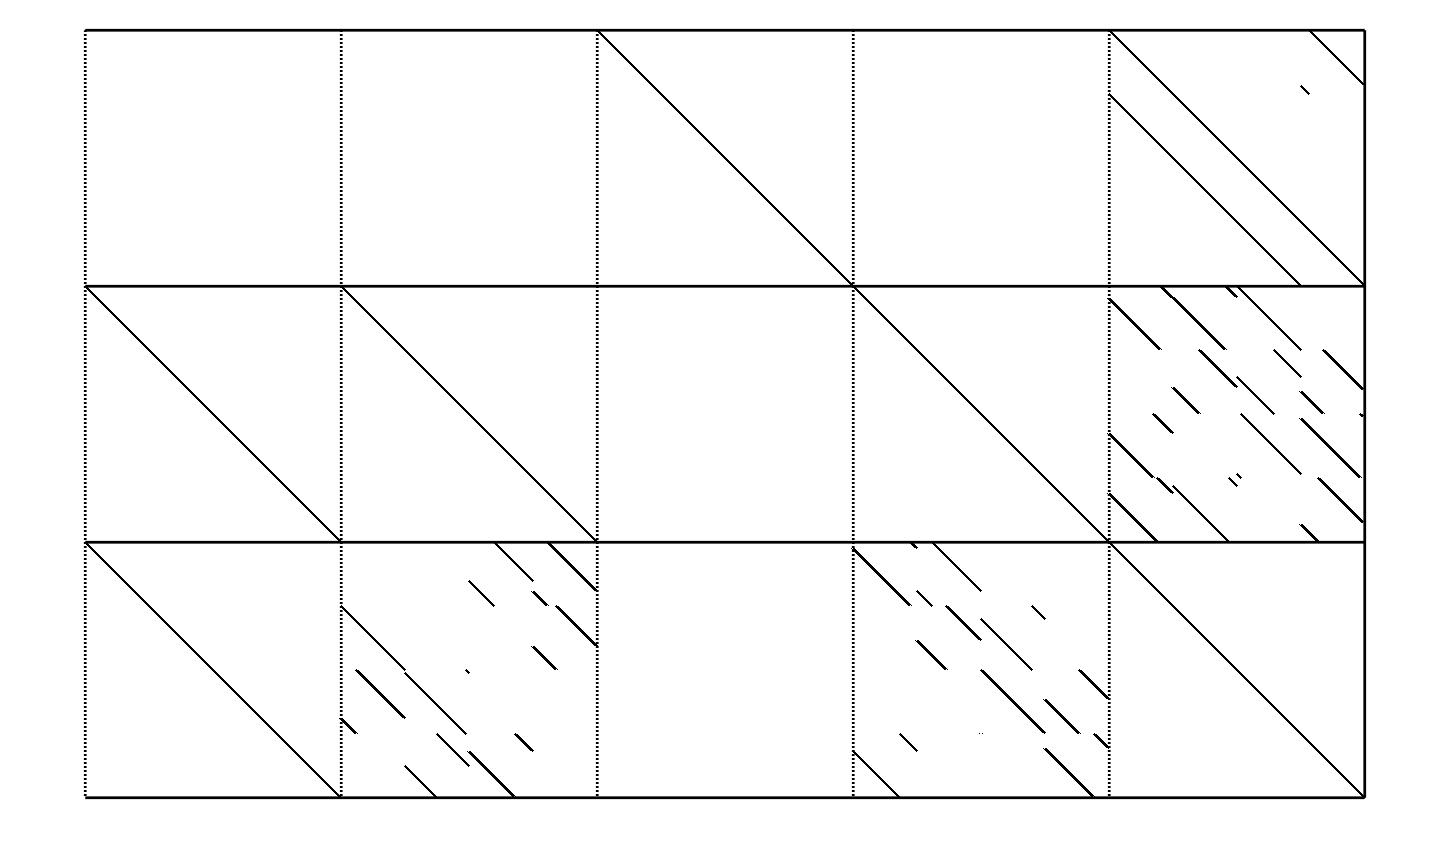
\includegraphics[width=0.4\linewidth]{Figures/HRUa.jpg}
                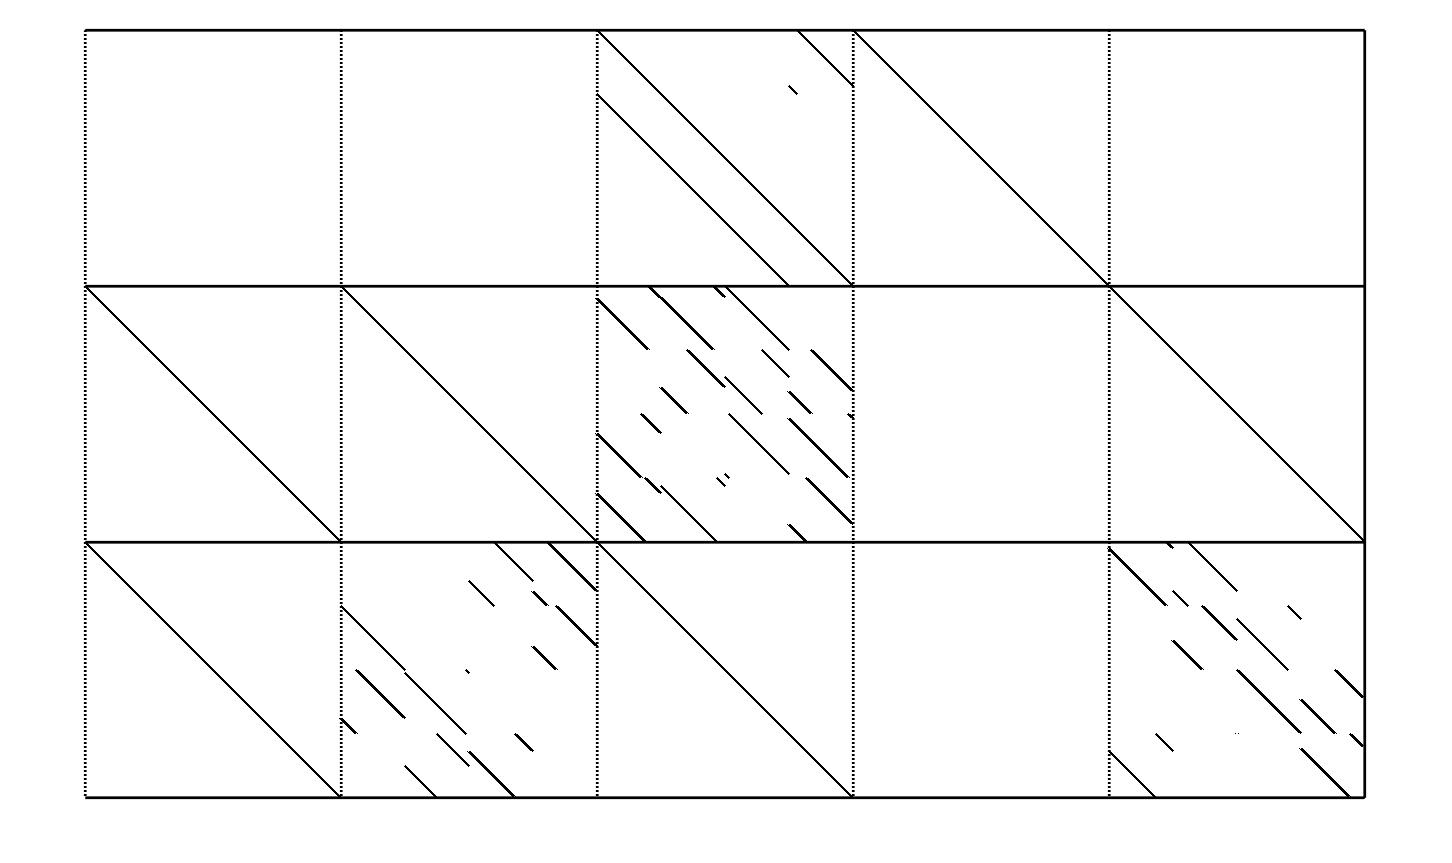
\includegraphics[width=0.4\linewidth]{Figures/HRUb.jpg}
                        \caption{$H$ matrix before (left) and after (right) the transformation into lower triangular form.}
                \label{fig:RUH}
                \end{figure}                    
        %       \begin{figure}
        %       \centering
        %       \includegraphics[width=0.3\linewidth]{Figures/phInv.png}
        %               \caption{$\varphi^{-1}$ submatrix for AR4JA codes $m=128$ bits for this code.}
        %       \label{fig:phiInv}
        %       \end{figure}    
            




\textbf{\textit{Partitioned $H$ methods}}\par
This class of methods is based on the fact that for all systematic codes, the codeword $c$ consists of the systematic part, which is a copy of the input information block and the parity bits: $c=\begin{bmatrix}s & p\end{bmatrix}$. The parity-check matrix can therefore be partitioned into a $(n-k)\times k$ submatrix $H_{1}$ and a $(n-k) \times (n-k)$ submatrix $H_{2}$, where $H=\begin{bmatrix}H_{1} & H_{2}\end{bmatrix}$, so that the parity bits vector can be calculated by (\ref{eq:H2inv1}), (\ref{eq:H2inv2}), (\ref{eq:H2inv2}).
    \begin{equation}
        Hc^{T}=H_{1}s^{T}+H_{2}p^{T}=0
        \label{eq:H2inv1}
    \end{equation}
    \begin{equation}
        H_{2}p^{T}=H_{1}s^{T}
        \label{eq:H2inv2}
    \end{equation}
    \begin{equation}
        p^{T}=H_{2}^{-1}H_{1}s^{T}
        \label{eq:H2inv3}
    \end{equation}
Submatrix $H_1$ is sparse and the vector $H_{1}s^{T}$ can be easily calculated. For many practical codes, submatrix $H_{2}^{-1}$ exhibits regular structure, which facilitates the involved calculations. A common structure in the parity-check matrix of many codes is the dual-diagonal: the rightmost part or of $H_{2}$, or even the entire submatrix (IEEE 802.11 n/ac, 3GPP2 DVB-S2) is a dual-diagonal matrix. \par
According to a variation of this method (\cite{Jia-ningSu2005}, \cite{Kaji2006}), $H_2$ matrix is decomposed into a permutation matrix $\Pi$ and two triangular matrices $L$, $U$, using triangular factorization (or LU decomposition).  Equation (\ref{eq:H2inv2}) is therefore transformed into (\ref{eq:LUH2-2}), from which parity bits are calculated using back-forward substitution. Conversely, the LU decomposition can be applied on $H_{2}^{-1}$ matrix, so that parity bits are calculated according to (\ref{eq:LUH2inv-1}),(\ref{eq:LUH2inv-2}).
                \begin{equation}        
                        H_{2}=\Pi^{-1}(LU)              
                        \label{eq:LUH2-1}
                 \end{equation}                                          
                 \begin{equation}
                         L[U(p^{T})]=\Pi(H_{1}s^{T})
                        \label{eq:LUH2-2}
                 \end{equation}  
                 \begin{equation}       
                        H_{2}^{-1}=\Pi'^{-1}(L'U')              
                        \label{eq:LUH2inv-1}
                 \end{equation}  
                 \begin{equation}
                        \Pi' p^{T}=L'[U'(H_{1}s^{T})]
                        \label{eq:LUH2inv-2}
                 \end{equation}
 The architectures proposed in \cite{Gomes2007}, \cite{AlHariri2013}, \cite{ZhiyongHe2006}, \cite{Hariri2014}, \cite{Perez2010a} and \cite{YongminJung2012} all follow algorithmically equivalent approaches which assume a dual-diagonal $H_2$ matrix. Parity bits can be calculated directly from the vector $H_{1}s^{T}$ using backward substitution. In  (\ref{eq:H2inv3}), $H_{2}^{-1}$ is a lower triangular matrix and $H_{2}^{-1}(i,j)=1, i\geq j$, so that back substitution is applicable.\par
For another class of codes (for example in IEEE 802.16e), $H_2^{-1}$ has the approximate dual-diagonal structure of (\ref{eq:ApproxDual}), where $I_{i}^{(x_{j})}$ are permutation matrices. Targeting these cases, \cite{Neto2015}, \cite{Kopparthi2007} and \cite{Chia-YuLin2008} propose  encoders with similar algorithmical description, which perform necessary permutations along with backward substitution for the calculation of the coresponding parity bits.\par         
    \begin{equation}
        H_{2}^{-1}=\left[
        \begin{array}{c|ccccc}
        I_{1}^{(x_{1})} & I & I & \dots &       0    & 0\\
        \vdots & & & \dots \\
        I_{b}^{(x_{b})} & 0 & 0 & \dots & I & I\\
        \end{array}\right]
    \label{eq:ApproxDual}
    \end{equation}\par
For many codes however (including those in \cite{CCSDS131.0}), $H_{2}^{-1}$ matrix has the structure of (\ref{eq:H2InvStruct}), where $0_{4m}$ and $I_{4m}$ are the $4m \times 4m$ zero and identity matrices and $W_{i,j}$ are $m \times m$ dense circulants, which is obviously not dual-diagonal, rendering the above architectures altogether inapplicable.
    \begin{equation}
        H_{2}^{-1}=
        \begin{bmatrix}
            I_{4m} & W_{1,1} & \dots  & W_{1,8} \\
            0_{4m} & \vdots  & \ddots & \vdots \\
            0_{4m} & W_{12,1} & \dots  & W_{12,8}
        \end{bmatrix}
        \label{eq:H2InvStruct}                  
    \end{equation}\par
The variation of the method based on L-U decomposition of $H_{2}$ according to (\ref{eq:LUH2-1})-(\ref{eq:LUH2inv-2}) is used in \cite{Jia-ningSu2005}, where the authors also propose an offline preprocessor for the triangulation of $H_{2}$. The QC structure of the matrix however is not kept in the decomposed matrices, at least for the demonstrated codes. Reference \cite{XiangranSun2011} proposes the same encoder architecture with a different decomposition algorithm for CMMB codes, which are not QC. The same encoder architecture is also proposed for CMMB in \cite{Wang2008}, without details on the decomposition algorithm. The work in \cite{Kaji2006} targets random Gallager codes. The encoding process is identical to \cite{Jia-ningSu2005}, however algorithms are provided for the calculation of permutation matrices, which minimize the density of $L$, $U$ components. It is shown that the compression achieved for the storage of sparse $L$, $U$ matrices favors this method over R-U, at least for Gallager codes. The adoption of this encoding method however for CCSDS inflicts a major performance penalty because of the loss of QC structure in $L$, $U$ matrices. For example, using the triangulation process outlined in \cite{Jia-ningSu2005}, the AR4JA rate $1/2$ code with $k$=1024 bits calls for the storage, proper indexing and processing of a total of around 64K nonzero elements of $L$, $U$ matrices, compared to the simple storage of the 2K elements of the first rows of the circulants needed for the $4m \times 4m$ $\varphi^{-1}$ matrix.\par               
The work in \cite{Mahdi2014} modifies the procedure in \cite{Jia-ningSu2005} and adopts LU decomposition of $H_{2}^{-1}$, so that parity bits are calculated according to (\ref{eq:LUH2inv-2}). It is shown that for the selected codes (Multi-level QC-LDPC codes), this method can result in more efficient storage of $L'$, $U'$ and $\Pi'$ in the encoder's memory than $H_{2}^{-1}$ or storing the components of $H_{2}$ according to \cite{Chia-YuLin2008}. However, the efficiency of the proposed encoding scheme is limited only to the two-step expanded codes, which results in cyclic structure in the triangulated components. Fig.\ref{fig:Mahdi-LU} depicts an example of the generated $L'$ and $U'$ matrices, compared to their CCSDS equivalents. The VMM architectures proposed for the vector-matrix multiplications are evidently not applicable for the random matrices of CCSDS. Memory requirements for indexing the non-zero values are also a considerable drawback. Another fully parallel method is also proposed, targeting high throughput. According to this method, there is no need to store $L'$, $U'$ in memory and the vector-matrix multiplications of (\ref{eq:LUH2inv-2}) are executed in parallel on all bits. This method cannot scale for higher block lengths or other codes. Even for CCSDS AR4JA $k$=1024, rate $1/2$ code, the implementation of this method required more than 72K LUTs, fitting only high-end Virtex 5 FPGAs, with prohibitive routing delays for any practical application.\par
\begin{figure}
    \centering
    
\includegraphics[width=0.24\linewidth]{Figures/LMahdi.png}
    
\includegraphics[width=0.24\linewidth]{Figures/UMahdi.png}
    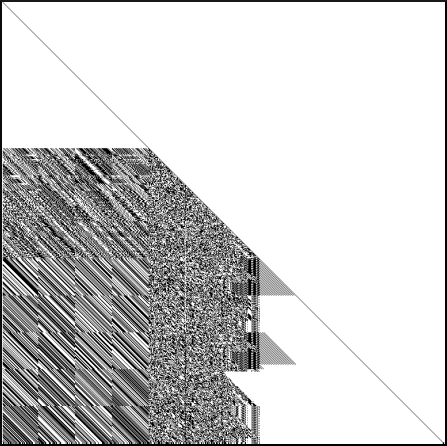
\includegraphics[width=0.24\linewidth]{Figures/LAR4JA.png}
    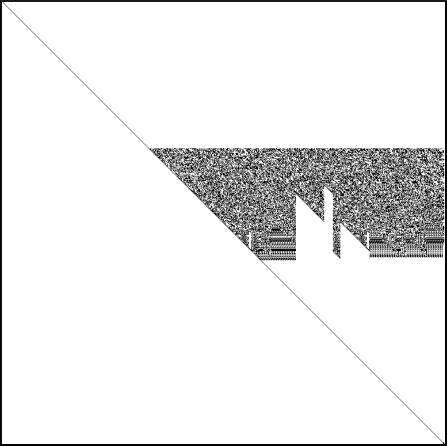
\includegraphics[width=0.24\linewidth]{Figures/UAR4JA.png}
    \caption{$L'$, $U'$ matrices of (2016,1008) example code in \cite{Mahdi2014} (left) and AR4JA $k$=1024 rate $1/2$ code (right).}
    \label{fig:Mahdi-LU}
\end{figure}    
In \cite{Cohen2009} the authors propose a hybrid approach, according to which the parity-check matrix is transformed in approximate lower-triangular form, as in R-U method. The parity bits are calculated using a mix of the direct and the R-U method: The first subvector $p_{1}$ of $g$ parity bits in R-U equation (\ref{eq:RU1}) is calculated from the the generator matrix $G$, according to the direct method. In this case, only the first $g$ columns of the submatrix $W_{n-k}$ in (\ref{eq:Wstructure}) need to be stored in encoder memory, avoiding thus the dense vector-matrix operations involving $\varphi^{-1}$. The paper focuses in IEEE 802.11an codes. For CCSDS AR4JA codes however, $g=4m$ and parameter $r$ is 8, 16, 32 for rates $1/2$, $2/3$, $3/4$ correspondingly, while $\varphi^{-1}$ is always $4m \times 4m$. No performance gain is therefore achievable from this method for CCSDS codes. On the contrary, memory requirements and critical path are adversely affected from the larger dense matrix involved. Also $T^{-1}$ is the identity matrix for AR4JA and the critical path is not affected.
                


\subsection{Packet level erasure codes}
Packet-level erasure coding has been proposed for many modern applications, such as edge computing \cite{Liang2020}, underwater acoustic sensor networks \cite{Geethu2015}, magnetic recording media \cite{Han2005}, hybrid broadcasting broadband television (HbbTV) \cite{Mattoussi2019} and delay tolerant networks (DTN) over deep space communication systems \cite{Alessi2020}. Joint use of erasure coding and bit-level FEC schemes in different scenarios has been studied in \cite{Courtade2011, Ostovari2015, Berger2008}.\par
The main focus of this thesis is on the implementation of encoders for the codes defined in \cite{CCSDS131.5}. The only implementation of the proposed codes is their integration into the the Interplanetary Overlay Network (ION) software suite \cite{ion}, which is a software implementation of the bundle protocol for Delay Tolerant Networks (DTN). In \cite{Alessi2020}, a multithreaded implementation of the ION libraries is proposed for better performance. However, the purely software approach proposed is expected to exert considerable strain on the on-board general purpose processor and mass memory subsystem of a space Software Defined Radio (SDR), which is typically responsible for these functions. Offloading these tasks to a small footprint hardware accelerator integrated into a FPGA is especially important in the case of microsats and cubesats and high data rate optical communications, to achieve reduced size, weight, power, and cost (SWaP-C). Typically, spacecraft subsystems already include FPGAs responsible for command and data handling (C\&DH) tasks and the recent trend is to fully utilize these devices for multiple combined functions \cite{Davarian2020}. Moreover, FPGA hardware acceleration of packet-level coding enables a very high speed data processing chain providing data rates in the scale of several Gbps.\par

\clearpage
\section{Goal of Thesis}
\label{sec:goal}
In the proposed thesis, I provide my research results on hardware implementations of encoders for the two cases described above: QC LDPC codes with no specific structure (other than QC) in the parity check matrix and the packet level erasure codes defined in \cite{CCSDS131.5}.
Regarding bit-level LDPC codes, my work introduces a novel solution, optimized for the codes of \cite{CCSDS131.0}, the most important feature of which is the efficient bit vector multiplication with dense matrices. Such multiplications are key operations for all LDPC encoding methods. This solution enables the design of novel encoder architectures and the resulting hardware implementations can achieve throughput performance in the range of multiple Gbps, with low resource utilisation. A lot of discussion is taking place lately about the endorsement of the rate $1/2$ LDPC codes of \cite{CCSDS131.0} into the new optical space communication standards \cite{CCSDS141}. The required performance however of the LDPC encoding and decoding components of the codec remains a challenging task and an active research area.\par
At the same time, the current work is the first approach to examine packet-level encoding algorithms and propose, implement and test hardware encoder architectures for these algorithms. Since their introduction in \cite{CCSDS131.5}, the proposed codes have not matured into a CCSDS recommended ("blue") standard yet. With the current research, I support that they can be placed among the options for modern high speed communications.\par
The theoretical results and analytical estimations are in all cases backed by active development and implementations on FPGA and MPSoC hardware, which also include validation and verification procedures: the proposed architectures are implemented as IP cores on the targeted platforms and their responses are compared against a bit-accurate software model, written in C or GNU/Octave. This development and testing process accounts for a significant part of the total research effort and calls for solid understanding and proficient use of the corresponding tools:
\begin{itemize}
    \item Xilinx Vivado
    \item Mentor Graphins Modelsim simulator
    \item Synopsis Synplify
    \item Vunit framework \cite{Vunit21}
    \item GNU/Octave language, which is the open-source equivalent of Mathworks Matlab
\end{itemize}
The DSCAL equipment available to support the research includes all the above listed software and a variety of development boards, including the XUPv5, Zedboard, ZC706 and ZCU102 boards.
\clearpage
\bibliographystyle{IEEEtran}
{\small 
\bibliography{library.bib}
}

\end{document}
